


\section{SafetyNet} \label{sec:safetynet}

\begin{table*}[t]
\centering
\input{ICLR25/table/benchmarking_anthropic}
\caption{Cross-dataset evaluation on MAD and Anthropic benchmarks. On MAD, \textsc{SafetyNet} achieves 97--100\% detection accuracy with perfect AUROC. On Anthropic, all methods struggle due to minimal separation between normal and harmful activation distributions (see Section~\ref{sec:limitations}). Beatrix shows consistent behavior across obfuscation conditions as it uses spectral features not targeted by our obfuscation loss. CROW exhibits high model-dependent variance on Anthropic.}
\label{tab:main}
\end{table*}

Based on our red-team findings that models exploit geometric shifting and covariate manipulation to evade detection (Section~\ref{sec:red_team}), we introduce SafetyNet---an ensemble detector designed to monitor multiple representational subspaces simultaneously. We hypothesize that harmful prompts trigger distinctly different reasoning patterns in the internal states of neural networks compared to normal responses, and that these differences manifest as outlier patterns in attention mechanisms and layer activations detectable through statistical and representational analysis.

\subsection{Attention-Based Feature Extraction} \label{sec:feature_extraction}

Using the notation introduced in Section~\ref{sec:red_team}, we extract the row-wise min-max normalized attention matrix $A_{\text{norm,row}}^l$ at the discriminative layer $l$ as the input feature for all detectors. All detectors are trained exclusively on benign attention patterns and identify harmful behaviors as out-of-distribution samples.

\subsection{Detector Ensemble} \label{sec:detectors}

SafetyNet combines four complementary detection methods targeting different geometric properties.

\paragraph{Autoencoder (AE).} Detects anomalies through reconstruction error, capturing non-linear manifold structure. The encoder maps the input through two hidden layers ($\text{input\_dim} \rightarrow 2048 \rightarrow 1024 \rightarrow 512$) with ReLU activations; the decoder mirrors this architecture. Trained with MSE reconstruction loss on benign samples, harmful inputs produce higher reconstruction error as they lie off the learned manifold.

\paragraph{Variational Autoencoder (VAE).} Captures probabilistic variations in latent space through Gaussian sampling, providing robustness against adversarial perturbations that might fool deterministic reconstructions. The architecture mirrors the AE but adds a reparameterization layer with learned mean and log-variance. The loss combines MSE reconstruction with KL divergence weighted by $\beta = 0.1$.

\paragraph{PCA (Linear Subspace).} Projects attention patterns onto the top 100 principal components fitted on benign data and computes the L2 distance from the projected mean. Our red-team experiments revealed obfuscated models often shift information into linear subspaces when evading non-linear detectors, making this detector complementary to AE/VAE.

\paragraph{Mahalanobis Distance (Covariance).} Computes the Mahalanobis distance using the sample mean and covariance estimated from benign data, with Tikhonov regularization ($\epsilon = 10^{-6}$) for numerical stability. This detector captures covariance anomalies that arise when models manipulate individual feature values while attempting to preserve overall statistics.


\begin{figure}[t]
    \centering
    
\includegraphics[width=\columnwidth]{figures/llama2_obfuscated_ae_detectors_comparison_layer_15_16.pdf}
    \caption{\textbf{Autoencoder robustness under obfuscation attack (Llama-3, MAD dataset).} Reconstruction loss distributions for normal (blue) and backdoored (red) samples. Despite adversarial training targeting autoencoder similarity, harmful samples exhibit clearly higher reconstruction losses, enabling reliable detection.}
    \label{fig:obfuscated_ae_mad}
    \vspace{-8pt}
\end{figure}


\subsection{Aggregation Strategy} \label{sec:aggregation}

The overall ensemble accuracy is computed using an ``any'' voting scheme: a sample is classified as harmful if \emph{any} detector in the ensemble flags it above threshold. For neural network detectors (AE/VAE), thresholds are set at $\mu + 2\sigma$ of the validation reconstruction losses; for distance-based detectors (PCA/Mahalanobis), thresholds are set at $\mu + \alpha\sigma$ of the training distances, where $\alpha$ is a configurable scale factor. This flagging strategy maximizes recall at the cost of false positives, appropriate for safety-critical applications where missing a harmful sample is more costly than a false alarm.
The theoretical intuition is that evading all detectors simultaneously requires either: (1) degrading task performance by removing information necessary for both harmful behavior and detection, or (2) leaving detectable signatures in at least one geometric subspace due to the complementary coverage of our ensemble. We formalize this as Proposition~\ref{prop:tradeoff} in Section~\ref{sec:method}.

Figure~\ref{fig:obfuscated_ae_mad} shows the reconstruction loss distributions for Llama-3 on the MAD dataset under obfuscation attack. Despite adversarial training, the autoencoder maintains clear separation between normal and backdoored samples, with harmful samples exhibiting reconstruction losses 0.18--1.07 higher than normal samples. See Appendix~\ref{app:detection} for detailed per-model reconstruction loss distributions across all five model families.




\begin{figure*}[t]
    \centering
    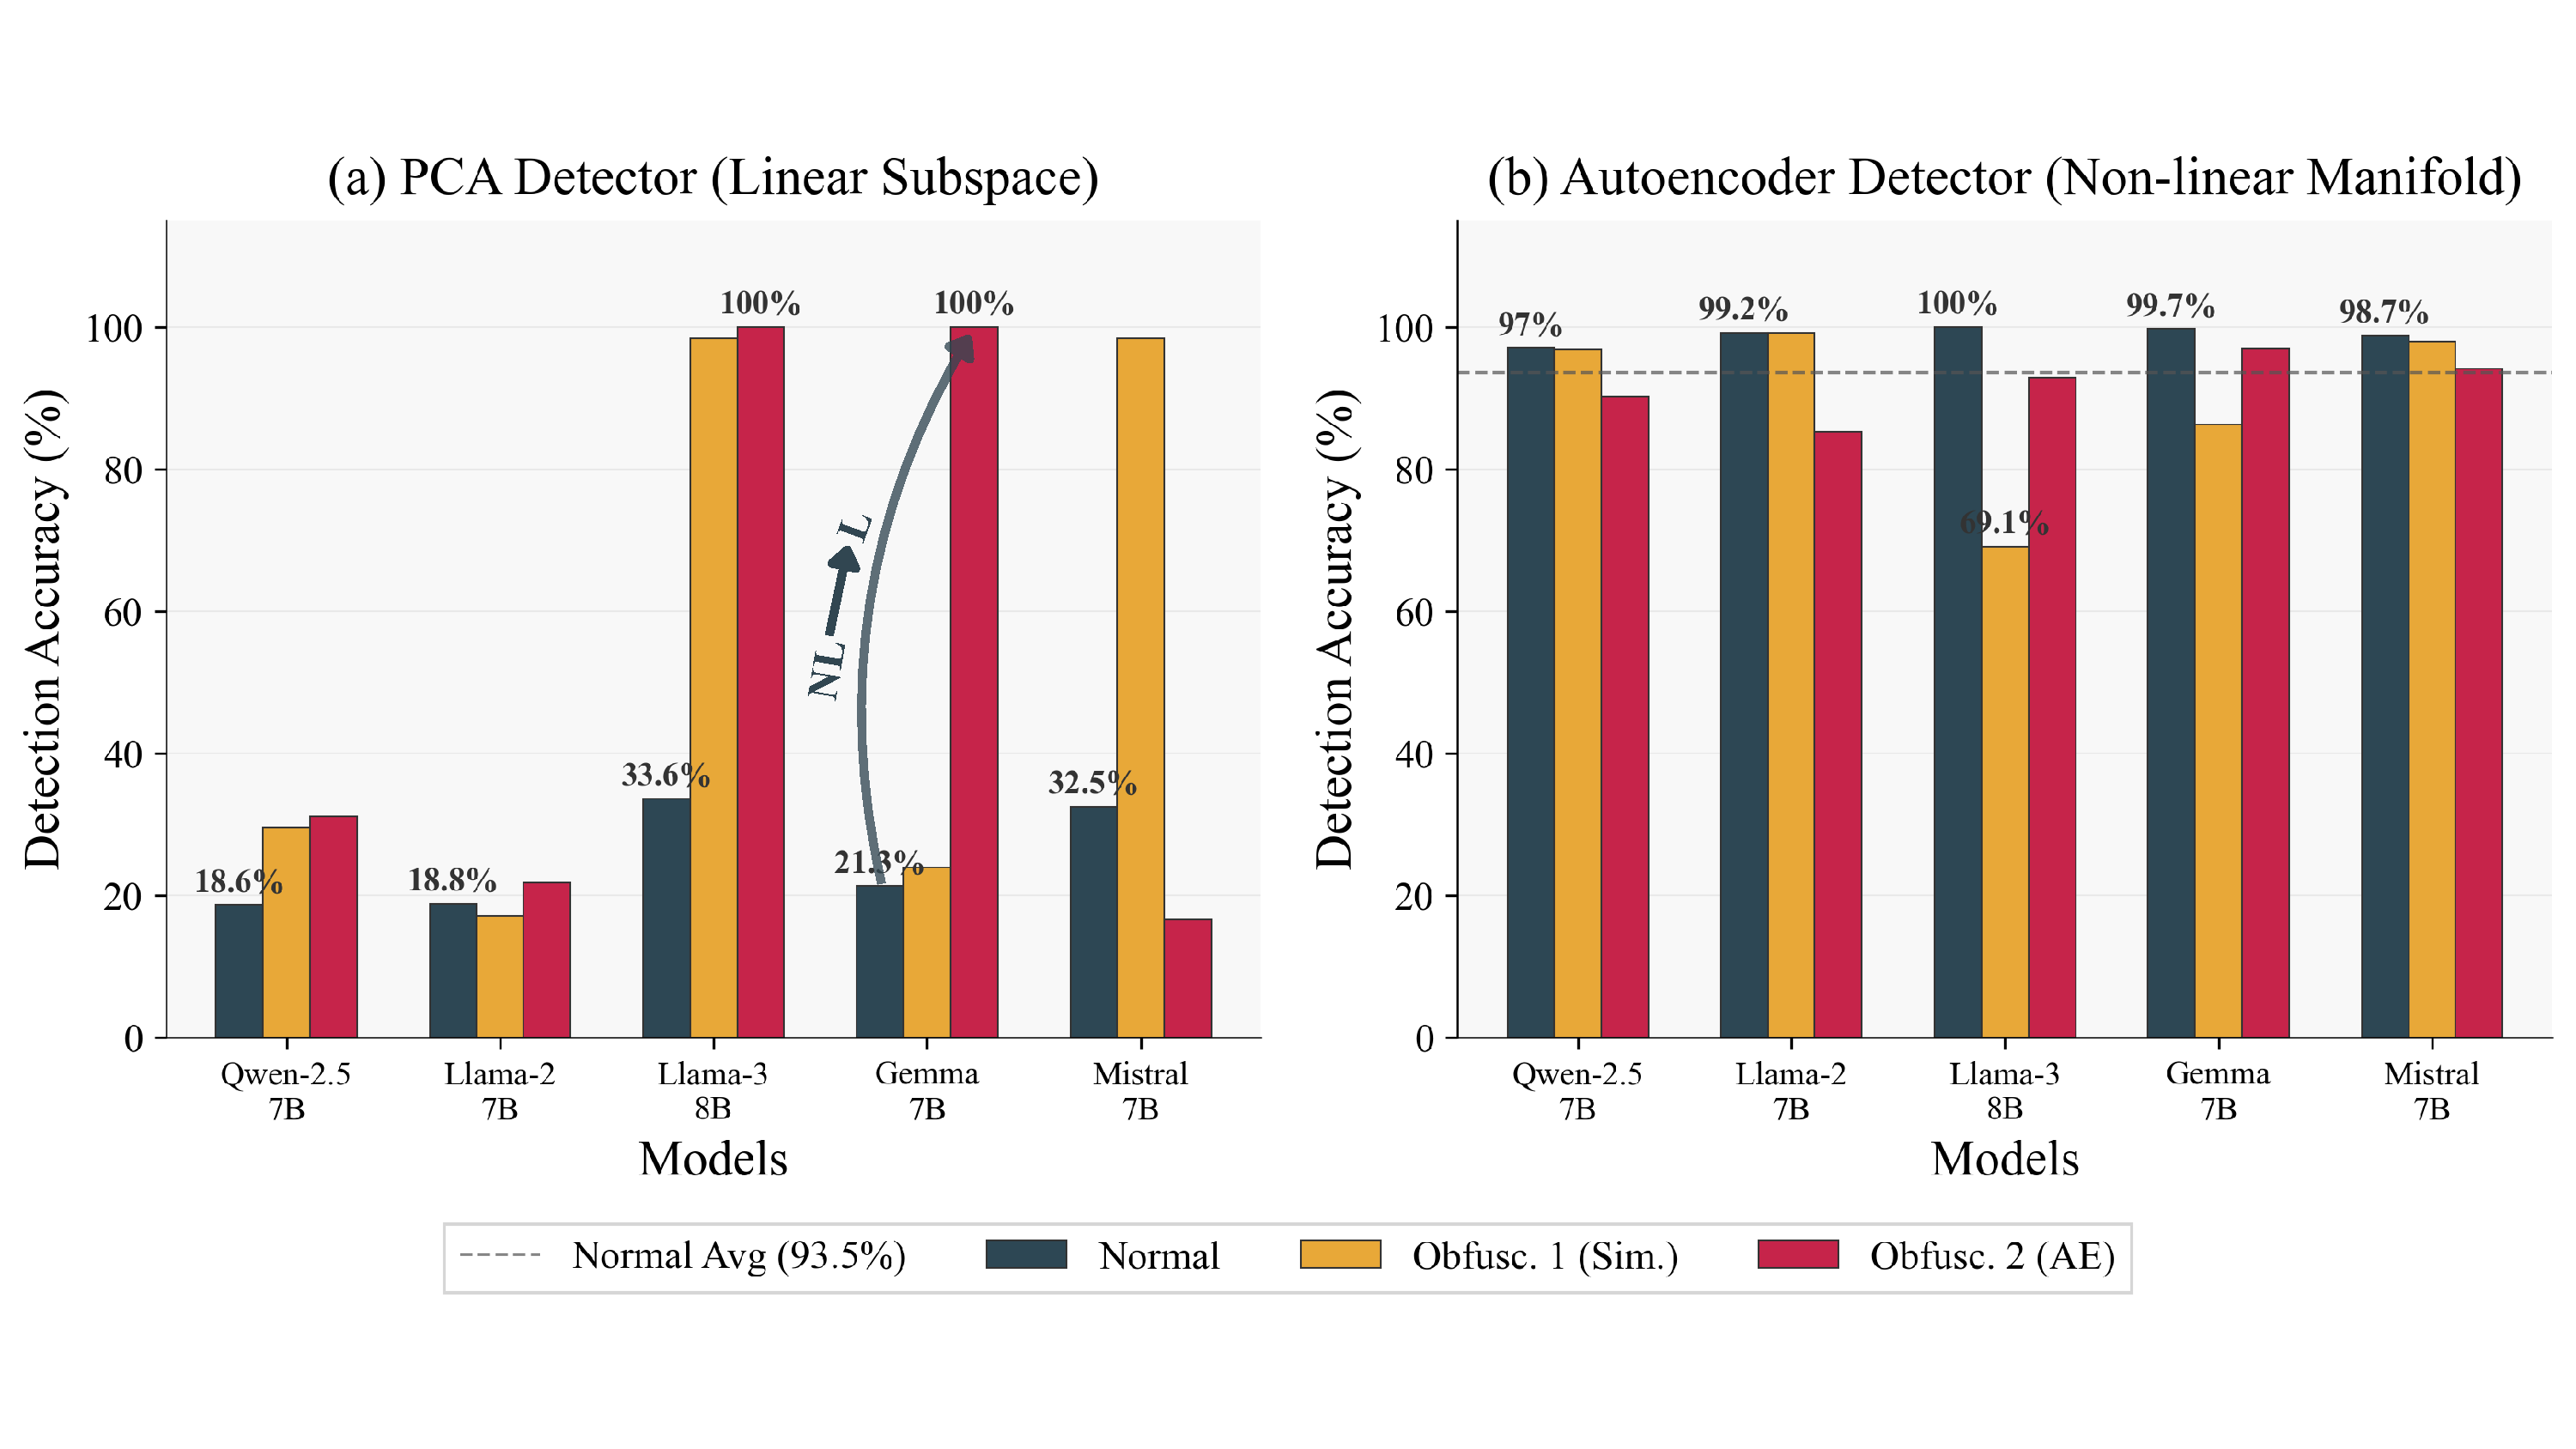
\includegraphics[width=0.85\textwidth]{figures/edited_geometric.pdf}
    \caption{\textbf{Geometric shifting between detector subspaces.} (a) PCA detector accuracy \textit{increases} dramatically under obfuscation (e.g., Llama-3: 33.6\% $\rightarrow$ 100\%), revealing information migration from non-linear space (NL) into linear space (L). (b) Autoencoder detector maintains high accuracy (85-100\%) even under direct AE attack, demonstrating non-linear manifold robustness. Arrows indicate geometric shifting---when models evade one detector type, they become detectable by the complementary detector.}
    \label{fig:geometric_shifting}
\end{figure*}
